% Metódy inžinierskej práce

\documentclass[10pt,twoside,slovak,a4paper]{article}


\usepackage[slovak]{babel}
%\usepackage[T1]{fontenc}
\usepackage[IL2]{fontenc} % lepšia sadzba písmena Ľ než v T1
\usepackage[utf8]{inputenc}
\usepackage{graphicx}
\usepackage{url} 
\usepackage{hyperref} 
\usepackage{}
%\usepackage{times}

\pagestyle{headings}

\title{Špirálový model a jeho použitie pri modelovaní softvéru\thanks{Semestrálny projekt v predmete Metódy inžinierskej práce, ak. rok 2021/22, vedenie: Ing. Vladislav Mlynarovič, PhD.}} 

\author{Tomáš Andel\\[2pt]
	{\small Slovenská technická univerzita v Bratislave}\\
	{\small Fakulta informatiky a informačných technológií}\\
	{\small \texttt{xandelt1@stuba.sk}}
	}

\date{\small 30. september 2021}



\begin{document}

\maketitle

\begin{abstract}
Špirálový model je metóda na vývoj softvéru. Vývoj pomocou tohto modelu sa vyznačuje tým, že kladie dôraz na redukciu rizík. Článok predstaví vývoj softvéru, niektoré tradičné modely, ich problémy a ako ich špirálový model rieši. Analyzuje postup vývoja pomocou špirálový modelu, porovná jeho výhody a nevýhody. Vysvetlí, prečo je analýza a riešenie rizík dôležité a ako ich tento model rieši. Ukáže ako veľa sa dnes využíva a predstaví konkrétny príklad využitia.

\paragraph{Kľúčové slová}: špirálový model, SDLC, vývoj softvéru, softvérové modelovanie, riešenie rizík
\end{abstract}

\section{Úvod}

Vývoj softvéru je zložitý proces. Tvorba nápadu, určenie požiadaviek, dizajn, implementácia, testovanie, údržba - tieto všetky a ďalšie procesy nastávajú pri vývoji softvéru, bez jasného plánu môže byť vývoj zdĺhavý a drahý. Už od možnosti vývoja prvého softvéru ľudia hľadajú modely, podľa ktorých budú pracovať, a ktoré im umožnia efektívne vyvíjať komplexné softvéry.

Existuje množstvo vývojových modelov, niektoré sú vhodnejšie na menšie projekty, pričom sú nepoužiteľné vo veľkých, kde by vývoj postupoval neefektívnym spôsobom. Iné sú zasa vhodnejšie na veľké projekty, ale pri malých projektoch by bolo ich použitie zbytočne komplikované. Tento článok ukáže vývoj skôr veľkých projektov a prečo je na to výbornou voľbou práve špirálový model.

V časti \ref{vyvojSoftveru} sa pozrieme na životný cyklus vývoja softvéru a aké fázy obnáša. V časti \ref{metody:vyvojSoftveru} bude predstavených niekoľko tradičných vývojových modelov a budú ukázané ich nevýhody a ako ich špirálový model rieši. V ďalšej časti (\ref{spiralModel}) prejdeme na samotný špirálový model. Ukážeme si ako funguje, aké sú jeho výhody/nevýhody v časti \ref{prosCons:spiralModel}, ako prebieha riešenie objavených rizík v časti \ref{risks:spiralModel}, kde a ako veľa sa využíva v časti \ref{usage:spiralModel}. Na záver sa ešte vyjadrím k témam z prednášok (\ref{reakciaNaTemy}) a v časti \ref{zaver} budú zhrnuté získané poznatky.

\section{Vývoj softvéru} \label{vyvojSoftveru}

Softvéroví inžinieri sa vždy snažia vyprodukovať kvalitný produkt, ktorý zodpovedá požiadavkám klienta, neprekročí pridelený rozpočet a je vyprodukovaný načas. Bohužial, často tieto ciele nie sú dosiahnuté. Ale dobrý manažment projektu vo vhodnom prostredí, ktoré sa drží zaužívaných metód a modelov môže zaručiť konzistené dosahovanie týchto cielov. \cite{Methodologies}

Životný cyklus vývoja softvéru je proces tvorby softvéru, ktorého cieľom je finálny produkt čo najvyššej kvality a čo najnižšej ceny \cite{SDLCdef}. Väčšinou obnáša tieto fázy:\cite{SDCLphases}
\begin{sloppypar}
\begin{enumerate}
\item \textbf{Iniciácia/Počiatočné plánovanie} - Diskusia o realizovateľnosti projektu, počiatočná estimácia nákladov a časovej náročnosti.
\item \textbf{Analýza požiadaviek a špecifikácia} - Identifikácia problémov, ktoré má vyvíjaný softvér riešiť a ich špecifikácia. Riešenie jeho operačných schopností, výkonostných charakteristík a infraštruktúry potrebnej na jeho údržbu.
\item \textbf{Funkčná špecifikácia alebo prototypovanie} - Identifikácia objektov, ich vlastností a vzťahov. Identifikácia obmedzení, ktoré obmedzujú správanie systému aťd. 
\item \textbf{Rozdelenie systémov (Build vs. Buy vs. Reuse)} - Rozdelenie systému na menšie časti a zistenie, ktoré časti je výhodné vyrobiť, ktoré stačí odkúpiť a nakonfigurovať k požiadavkám systému, a ktoré je možné opäť použiť z predošlých projektov.
\item \textbf{Architektúra} - Definuje prepojenia a vytvára rozhrania medzi jednotlivými podsystémami, komponentami a modulmi aby bol možný ich jednotlivý detailný dizajn.
\item \textbf{Detailný dizajn komponentov} - Definuje funkciu jednotlivých komponentov, ich interné správanie, ako transformujú vstupy na požadované výstupy.
\item \textbf{Implementácia komponentov} - Kodifikuje špecifikácie navrhnuté počas architektúry a detailného dizajnu komponentov do funkčného zdrojového kódu.
\item \textbf{Testovanie a kontrola integrity} - Kontrola systému a podsystémov na základe ich požiadaviek. Kontroluje celkovú integritu systému.
\item \textbf{Tvorba dokumentácie} - Vytváranie systematických dokumentov a užívateľských príručiek.
\item \textbf{Spustenie softvéru pre klienta/užívateľa} - Poskytnutie softvéru užívatelovi a prípadne inštrukcie na inštaláciu a konfiguráciu.
\item \textbf{Školenie a používanie softvéru} - Školenie užívateľov systému ako správne a efektívne softvér využívať.
\item \textbf{Údržba softvéru} - Udržiavanie operatívnosti softvéru, opravovaním objavených chýb, poskytovaním funkčných alebo výkonnostných vylepšení a údržbou podpornej infraštruktúry.
\end{enumerate}
\end{sloppypar}




\subsection{Metódy vývoja softvéru} \label{metody:vyvojSoftveru}
Metódy alebo modely na vývoj softvéru popisujú spôsob navigácie medzi vyššie uvedenými procesmi vývoja.\cite{ModelDef}

Existuje veľké množstvo modelov a každý z nich je vhodný v inej situácií. Pozrime sa na niekoľko tradičných modelov \cite{Methodologies}:
\begin{itemize}
\item \textbf{Waterfall Model} - Jeho grafická reprezentácia vyzerá ako kaskáda vodopádov. Je to jeden z najstarších modelov a je základom mnohých iných modelov. Pri používaní tohto modelu je každý proces najprv dokončený a až potom sa prechádza na ďalší. Jeho nevýhodou je nízka úroveň flexibility, všetky požiadavky je potrebné vedieť už na začiatku. Nie je vhodný na veľké projekty. Analýza rizík je často zložitá.
\item \textbf{Sashimi Model} - Waterfall model, pri ktorom je dovolená paralelná práca na viacerých fázach naraz, je časovo výhodnejší.
\item \textbf{V-Shaped Model} - Je považovaný za rozšírenie Waterfall modelu. Namiesto lineárneho pohybu nadol sa vytvára tvar V s vrcholom, v ktorom je implementačný proces. Model vytvára vzťahy medzi vývojovými procesmi pred implementáciou a ich príslušnými fázami testovania. Výhodou tohto modelu jednoduché použitie rovnako ako pri Waterfall modeli a narozdiel od Waterfall modelu je tu vyššia šanca úspechu kvôli plánovaniu testovania už na začiatku vývoja. Nevýhodou je nízka úroveň flexibility a nemožnosť tvorby skorých prototypov pretože celková produkcia kódu je až vo fáze implementácie.
\end{itemize}

Ako je možné vidieť, nevýhodami týchto modelov sú hlavne nízka flexibilita a zlá analýza rizík. Pri vývoji veľkých projektov častov vznikajú rôzne riziká, ktoré sa pri tých menších objavujú menej. Preto veľké firmy hľadajú iné modely, pomocou ktorých tieto riziká vedia odhaliť a uskutočniť určité kroky na ich spracovanie.

V ďalšej časti sa pozrieme na špirálový model a ako dokáže tieto problémy riešiť.

\pagebreak

\section{Špirálový model} \label{spiralModel}
Špirálový model, pôvodne navrhnutý Barrym W. Boehmom, je evolučný softvérový procesný model, ktorý spája iteračnú vlastnosť prototypovania s riadenými a systematickými aspektmi lineárneho sekvenčného modelu. \cite{SpiralModelDef}

Jeho diagram vyzerá ako špirála s mnohými sľučkami (viď. obrázok \ref{spiralDiagram}). Každá sľučka špirály sa nazýva fáza vývojového procesu softvéru. Presný počet fáz závisí od zložitosti projektu. Projektový manažér analyzuje riziká a iné faktory, podľa ktorých dynamicky určuje počet týchto fáz.

\begin{figure}[h]
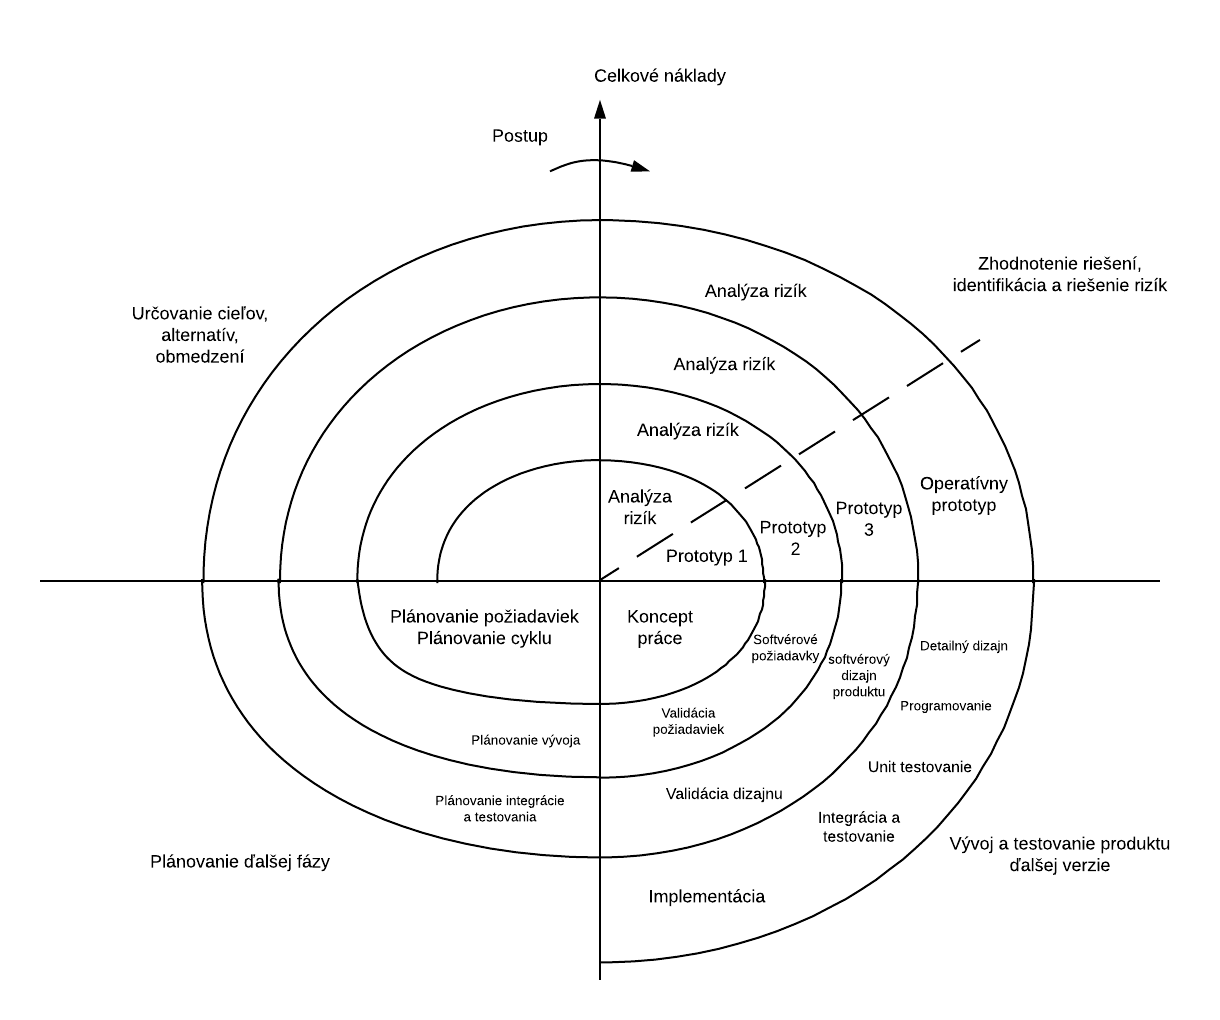
\includegraphics[width=\textwidth]{spiralModel.png}
\caption{Diagram špirálového modelu - upravené podľa \cite{Boehm}} 
\label{spiralDiagram}
\end{figure} 

Čím je väčší počet fáz, tým sú väčšie náklady projektu - polomer špirály predstavuje celkové náklady projektu. Uhol medzi pozorovaným miestom a začiatkom fázy predstavuje dosiahnutý postup v danej fáze. \cite{SpiralModelDef1}

Každá fáza je rozdelená do štyroch kvadrantov, ako je znázornené na obrázku. Kvadranty sú \cite{SpiralModelDef1}:
\begin{enumerate}
\item \textbf{Určovanie cieľov, alternatív, obmedzení } - V tomto kvadrante prebieha zbieranie požiadaviek od klientov, analýza a identifikácia cieľov a potom diskusia ohľadom alternatívnych riešení, ktoré by mohli byť použité v ďalších častiach súčasnej fázy.
\item \textbf{Zhodnotenie riešení, identifikácia a riešenie rizík } - V druhom kvadrante sú všetky možné riešenia zhodnotené a vyberie sa najlepšie riešenie. Ďalej prebieha analýza rizík spojených s vybraným riešením, tie sú následne riešené pomocou najvhodnejšej stratégie. Na konci tohto kvadrantu je zhotovený prototyp, ktorý je v súlade s vybranou najlepšou stratégiou.
\item \textbf{Vývoj a testovanie produktu ďalšej verzie} - V treťom kvadrante prebieha všetka implementácia a testovanie. Určené špecifikácie sú vytvárané a testované. Na konci tohto kvadrantu je pripravená ďalšia verzia produktu.
\item \textbf{Plánovanie ďalšej fázy} - Klient zhodnotí vytvorený produkt a prebieha plánovanie ďalšej fázy.
\end{enumerate}

\subsection{Výhody a nevýhody špirálového modelu} \label{prosCons:spiralModel}

Ako je zjavné z popisu vyššie, tento model je vhodný najmä pre rozsiahle, komplexné projekty. Progresívna povaha tohto modelu umožňuje vývojárom rozdeliť veľký projekt na menšie časti a venovať sa plne jednej funkcii, čo zaručuje lepšie prepracovanie, menší počet chýb atď. \cite{SpiralModelDef2} 

Medzi ďaľšie \textbf{výhody} špirálového modelu patrí \cite{SpiralModelProsCons} :
\begin{itemize}
\item Prvé verzie softvéru sú dostupné už na začiatku vývoja.
\item Riešenie rizík - je jednou z najdôležitejších predností špirálového modelu. Vďaka analýze a riešeniu rizík v každej fáze tento model minimalizuje riziko neúspechu rozsiahlych projektov.
\item Flexibilný vzhľadom na nové požiadavky - pri vývoji týmto modelom, môžeme kedykoľvek v neskorších fázach vývoja zmeniť požiadavky na vyvíjaný softvér a ľahko a správne ich zapracovať do softvéru. Rovnako môže byť kedykoľvek pridaná aj ďalšia funkcionalita.
\item Vývoj týmto modelom je otvorený spolupráci so zákazníkmi/užívateľmi. Zákazníkov môžeme, najmä vďaka tvorbe skorých a pravidelných prototypov, zapájať už od začiatku vývoja. Toto redukuje množstvo nedorozumení a tým šetrí čas a náklady na prerábanie nevhodnej funkcionality.
\item Kontrola postupu práce a tvorba dokumentácie je na vysokej úrovni.
\item Je vhodný pre vysoko rizikové projekty. Pomocou tohto modelu je možné vytvoriť veľmi prispôsobený produkt.
\end{itemize}

\bigskip

Medzi  \textbf{nevýhody} špirálového modelu patrí \cite{SpiralModelProsCons} :
\begin{itemize}
\item Nie je vhodný na malé projekty. Vývoj by bol moc nákladný a nedokázali by využiť jeho plný potenciál.
\item Vysoká komplexita - je komplexnejší ako väčšina ostatných vývojových modelov.
\item Dôraz na analýzu a riešenie rizík vytvára potrebu neštandardnej špecifickej expertízy.
\item Neurčité časové estimácie. Kedže počet fáz býva na začiatku vývoja neznámy, nie je jednoduché určiť časovú dĺžku vývoja softvéru, preto sa využíva skôr na dlhodobý vývoj.
\item Špirála sa môže pokračovať do nekonečna.
\item Nie je vhodný na nízko rizikové projekty. Pre takéto projekty nie je dôvod tento model využívať.
\item Definícia jasných, overiteľných miľníkov môže byť zložitá. Častá zmena funkcionality si vyžaduje nadmernú dokumentáciu.
\end{itemize}

\subsection{Riešenie rizík pomocou špirálového modelu} \label{risks:spiralModel}
Riziko je akákoľvek nepriaznivá situácia, ktorá môže ovplyvniť úspešné dokončenie softvérového projektu. Najdôležitejšou vlastnosťou špirálového modelu je analýza a riešenie týchto rizík. Takéto riešenia rizík sa dajú ľahšie vykonať vývojom prototypu. Špirálový model má na tento proces vyhradený jeden kvadrant v každej fáze vývoja.

Aj "prototypovací model" podporuje analýzu a riešenie rizík, ale všetky riziká musia byť identifikované už pred začatím vývoja. Avšak často sa riziká naskytávajú aj počas vývoja, takže v tomto je špirálový model flexibilnejší a celkovo vhodnejší. \cite{SpiralModelDef}


\subsection{Využitie špirálového modelu} \label{usage:spiralModel}
Dáta o popularite špirálového modelu sú ťažko dohľadateľné, takže v tejto téme som sa odrazil iba od jednej štúdie spoločnosti GoodFirms, preto môžu byť výsledky nepresné. 

V tejto štúdii GoodFirms skúmali 150 firiem, ktoré vyvíjajú softvér. Jedným z faktorov, ktorý skúmali je aké vývojové modeli tieto firmy využívali. Výsledky tohto prieskumu sú uvedené v tabuľke \ref{usageTab}

\begin{table}[!ht]
	\caption{Využitie vývojových modelov firmami \cite{SpiralModelUsage}}
	\label{usageTab}
    \centering
    \begin{tabular}{|l|l|l|l|l|l|l|l|l|l|}
    \hline   
    \hline
        Model           & Počet firiem & Podiel \\ \hline
    \hline
        Agile           & 92           & 61\%       \\ \hline
        Scrum           & 35           & 23\%      \\ \hline
        Waterfall       & 14           & 9\%      \\ \hline
        Špirálový a iné & 9            & 6\%      \\ \hline
    \hline
        Spolu           & 150            & 100\%     \\ \hline
    \end{tabular}
\end{table}

Ako je možné vidieť v tabuľke, táto štúdia naznačuje minimálne využitie špirálového modelu. Jedným z dôvodov môže byť nevhodná vzorka skúmaných firiem - v štúdii sa vyskytovali najmä menšie firmy, ktoré sa len zriedka púštajú do vývoja rozsiahlych projektov. Preto sa teraz pozrieme na konkrétny príklad využitia špirálového modelu.

\paragraph{GanttPRO} - Aplikácia, ktorá poskytuje nástroje na projektový manažment, podobná aplikáciám ako Notion alebo MS Project.

Vývojári využívali pri vývoji špirálové a scrum princípy. Napríklad kratšie iterácie, čo im dovolilo častejšie produkovať prototypy a tým získali častejšiu spätnú väzbu. Pre každú iteráciu (fázu) vytvorili detailný plán práce.

Hlavnými problémami, ktorým vývojári čelili, boli:
\begin{itemize}
\item Rôzne nové požiadavky, ktoré sa časom naskytovali. Z iterácie do iterácie ich bolo potrebné objasniť a zakomponovať.
\item Potreba analýzy a riešenia rizík, ktoré sa vývojom naskytovali.
\item Možné zvýšené náklady spôsobené dlhým plánovaním.
\end{itemize}
Zvolili teda kratšiu frekvenciu vývoja prototypov - dvojtýždňové iterácie. V dôsledku toho sa im podarilo zredukovať množstvo rizík a maximalizovať zisky vďaka rýchlemu prispôsobeniu sa potrebám používateľov a trhu. \cite{SpiralModelExample}

\subsection{Reakcia na témy z prednášok} \label{reakciaNaTemy}
V tejto časti zareagujem na niekoľko tém, ktoré boli obsahom prednášok na predmete MIP.

 \paragraph{Inžinierska gramotnosť} - V tejto prednáške sme sa dozvedeli kto je vlastne inžinier. Inžinier pracuje najmä s technickými informáciami - mal by vedieť pochopiť, interpretovať, aplikovať a ďalej odovzdať informáciu. Spomedzi viacerých zdrojov na rovnakú tému, by mal vedieť zhodnotiť čím a prečo sa odlišujú.

Ďalej sme sa dozvedeli o inžinierskej gramotnosti. Obnáša presné písomné alebo ústne vyjadrovanie, pričom používa prostriedky a nástroje, ktoré mu takéto vyjadrovanie umožnia. Jedným z takýchto nástrojov je LaTeX, o ktorom sme sa dozvedeli v zápätí. Tento nástroj sa zdá menej praktický ako WYSIWYG editory, ale po jeho používaní pri písaní článku som názoru, že nie je vôbec na zahodenie.

 \paragraph{Načo budem inžinierom?} - Túto prednášku prezentoval dekan fakulty, profesor Ivan Kotuliak. Rozprával napríklad prečo je vysokoškolské vzdelanie dôležité alebo o dôležitosti dokumentácie práce, s čím súhlasím. Pokračoval v predstavovaní rôznych možností zamestnania v IT a rôznych IT aplikáciách. Táto prednáška bola podľa môjho názoru zaujímavá a inšpiratívna.

\paragraph{Udržateľnosť a etika} - Táto prednáška sa zaoberala udržateľnosťou a pokladala otázku, či je možné udržať návštevnosť študentov na prednáškach. Myslím si, že do určitej miery to je možné. Najskôr sú tu radikálnejšie riešenia ako je povinná účasť alebo povinné skúšanie/testy na prednáške, tieto sú efektívne, ale vrámci udržania návštevnosti študentov z vlastnej vôle sú nevhodné. Iné riešenia môžu byť napríklad prednes dôležitých informácií, ktoré sa mimo prednášky nenachádzajú, interakcia so študentami alebo rôzne zaujímavé obmeny obsahu prednášky.

Ďalej sa prednáška zaoberala etikou - myslím si, že etické správanie je dôležité. Zvyšuje životnú úroveň a je dôležitou súčasťou modernej spoločnosti. Rovnako dôležité je aj v IT.

\section{Záver} \label{zaver} 
Článok stručne predstavil vývoj softvéru a životný cyklus vývoja softvéru. Ďalej, na porovnanie, priblížil pár základných metód (modelov) vývoja softvéru. V ďalších častiach bol spodrobnený špirálový model, práca s ním a riešenie rizík. Prieskum využitia špirálového modelu ukázal nízky záujem s čím nesúhlasím. Iné zdroje naznačujú rozsiahlejšie využitie tohto modelu, ale bez potrebných dát, ktoré by tieto tvrdenia potvrdzovali. 

V závere teda článok poskytol prehľad o špirálovom modeli vývoja softvéru, ukázal jeho prednosti a kedy ho je vhodné využívať.



\bibliography{literatura}
\bibliographystyle{abbrv}
\end{document}
